%\newpage
\section{D-Separation}\label{sec:d-sep}

From Section~\ref{sec:i-map}, we know that a graph structure $G$ encodes a set of conditional independence assumptions $I(G)$ and we can read a set of independencies directly according to the Markov assumption.  
However, we may be interested to infer all possible conditional independence from a graph $G$. 

\begin{definition}
D-separation is a procedure $\dsep_G(X\bot Y|Z)$ that, given a graph $G$ and three sets $X$, $Y$, and $Z$ of nodes in $G$,  returns Yes or No, such that $\dsep_G(X\bot Y|Z)=Yes$ iff $(X\bot Y|Z)$ follows from $I(G)$.
\end{definition}

First of all, we note that if $X$ and $Y$ are connected directly, they are co-related regardless of any evidence about any other variables. So, in the following, we consider $X$ and $Y$ that are not directly connected. 

\subsection{Four Local Triplets}

Before considering more complex cases, we consider  four local cases where $X$ and $Y$ are indirectly  connected with another variable $Z$ in the middle. The four possible cases are shown in Figure~\ref{fig:d-sep-simple}. 

\begin{figure}[!htbp]
    \centering
    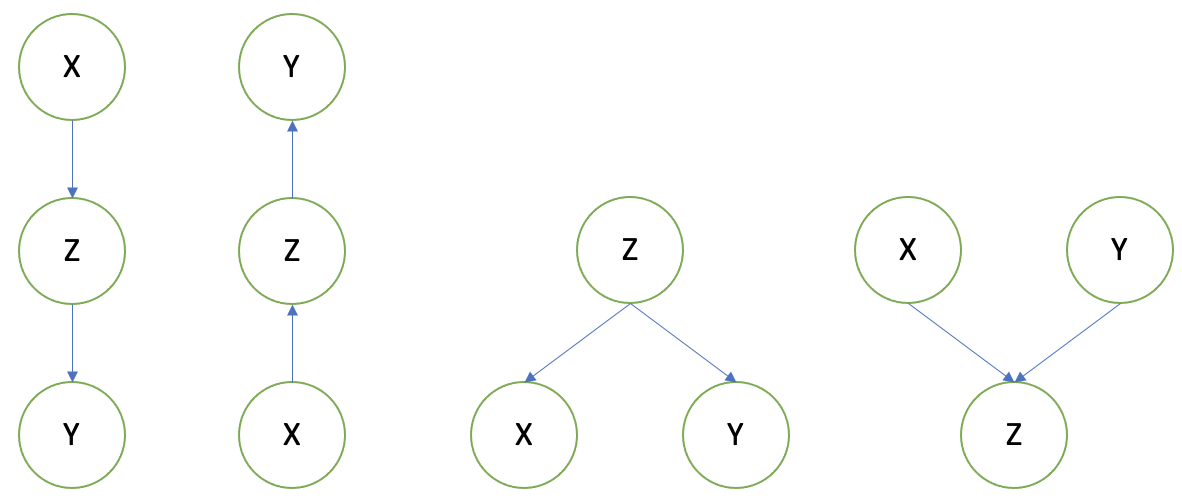
\includegraphics[width=0.6\textwidth]{images/graphical models/d-sep/d-sep-simple.png}
    \caption{Four patterns}
    \label{fig:d-sep-simple}
\end{figure}

\subsection*{Indirect Causal Effect $X\rightarrow Z\rightarrow Y$} 

Cause $X$ cannot influence effect $Y$ if $Z$ is observed, i.e.,  observed $Z$ blocks the influence of $X$ over $Y$. For the running example, as shown in Figure~\ref{fig:indirect-causal}, 


\begin{figure}[!htbp]
    \centering
    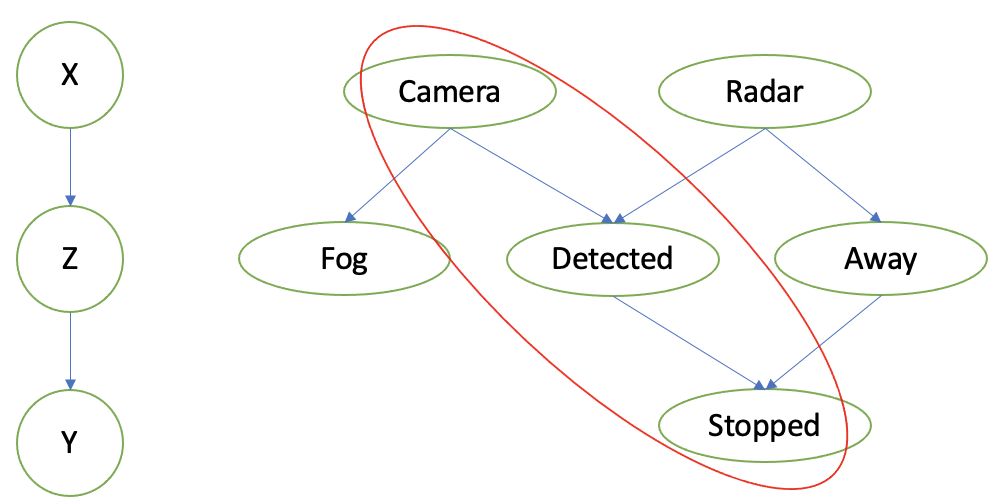
\includegraphics[width=0.5\textwidth]{images/graphical models/d-sep/indirect-causal.png}
    \caption{Indirect Causal Effect}
    \label{fig:indirect-causal}
\end{figure}

\subsection*{Indirect Evidential Effect $Y\rightarrow Z\rightarrow X$} Similarly, evidence $X$ cannot influence the cause $Y$ if $Z$ is observed. 


\subsection*{Common Cause $X\leftarrow Z\rightarrow Y$}

Once $Z$ is observed, one of the effects cannot influence the other.  Figure~\ref{fig:common-cause} presents a case of common cause in our running example. 

\begin{figure}[!htbp]
    \centering
    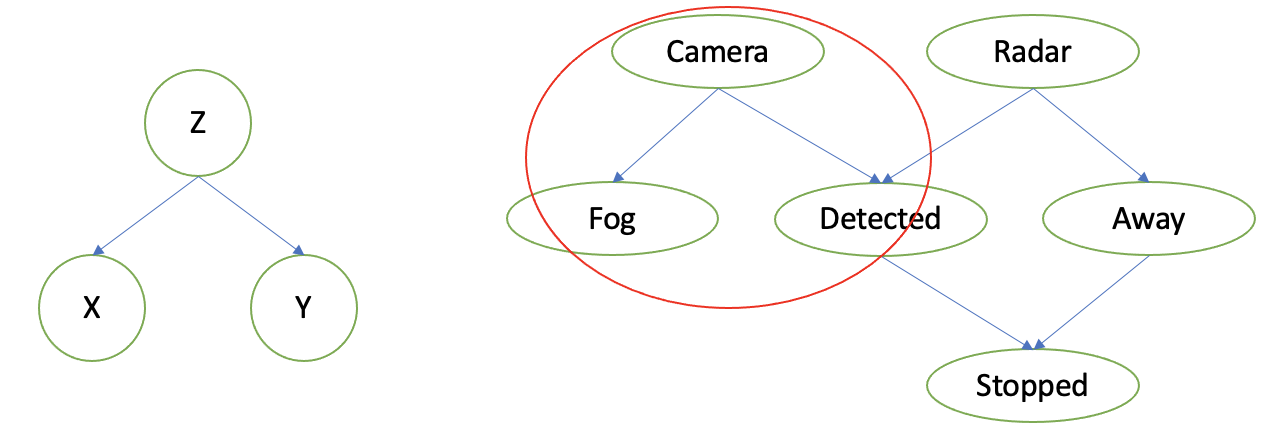
\includegraphics[width=0.6\textwidth]{images/graphical models/d-sep/common-cause.png}
    \caption{Common Cause}
    \label{fig:common-cause}
\end{figure}

\subsection*{Common Effect $X\rightarrow Z\leftarrow Y$} 

Unlike the above three cases where observing the middle variable $Z$ blocks the influence, the case of common effect is on the opposite, i.e., the influence is blocked when the common effect  $Z$  and its descendants are not observed. Figure~\ref{fig:common-effect} presents a case of common effect in our running example. 

\begin{figure}[!htbp]
    \centering
    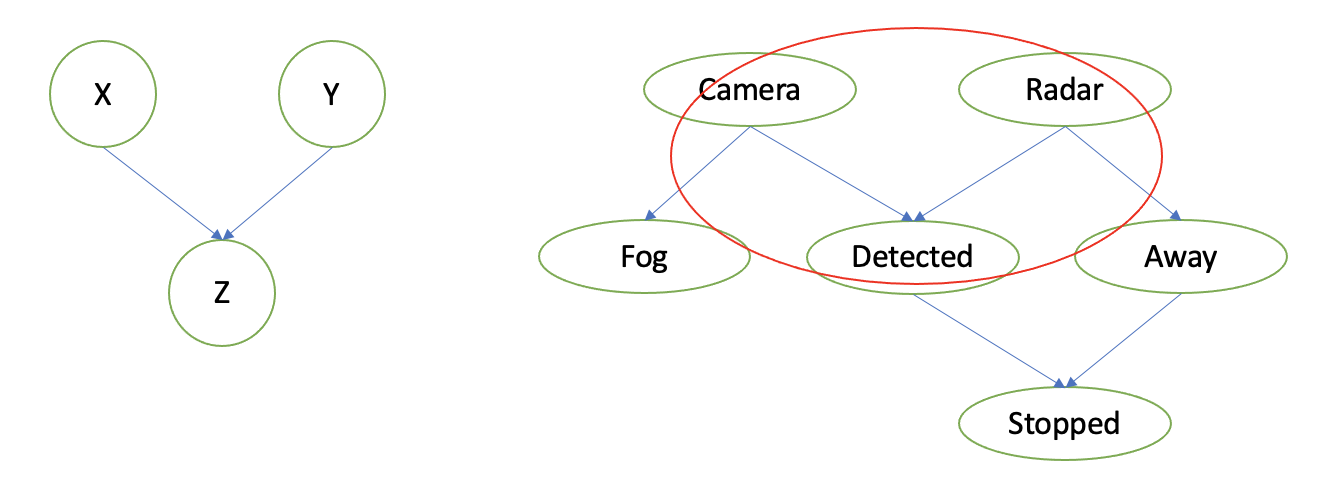
\includegraphics[width=0.6\textwidth]{images/graphical models/d-sep/common-effect.png}
    \caption{Common Effect}
    \label{fig:common-effect}
\end{figure}

\subsection{General Case: Active Trail and D-Separation}

Summarising the above discussion on local canonical cases (or v-structures), we have that 
\begin{itemize}
    \item Causal trail, $X\rightarrow Z\rightarrow Y$, is active if and only if $Z$ is not observed.  
    \item Evidential trail, $X\leftarrow Z\leftarrow Y$, is active if and only if  $Z$ is not observed. 
    \item Common cause, $X\leftarrow Z\rightarrow Y$, is active if and only if $Z$ is not observed. 
    \item Common effect, $X\rightarrow Z\leftarrow Y$, is active if and only if either $Z$ or one of its descendants is observed. 
\end{itemize}
%
Now we can consider the general case of $\dsep_G(X\bot Y|Z)$, where $X$, $Y$ and $Z$ may not be connected to each other. Actually, the graph can be large and the variables may be far away from each other. Fortunately, as we will introduce below, any complex case can be broken into repetitions of the local canonical cases. 

The D-separation algorithm is given in Algorithm~\ref{alg:dsepalg}. It collects all paths between $X$ and $Y$, without considering the directions of the edges. Then, as long as no paths are active given the observations $\{Z_1,...,Z_k\}$, the two variables $X$ and $Y$ are conditionally independent. 

\begin{algorithm}[!htbp]
\SetAlgoLined
%\KwResult{$S^0_i$ is the spike trains of input $X^0_i$}
\SetKwFunction{ConstructSubTree}{a set of training instances $D$}
$Path = $ all (undirected) paths from $X$ to $Y$ \\
\For{$path$ in $Path$}{
\eIf{isActive($path$, \{Z_1,...,Z_k\}) 
}{
\Return  $X\not\bot Y|\{Z_1,...,Z_k\}$
}
}
\Return $X\bot Y|\{Z_1,...,Z_k\}$
\caption{$\functionname{d-sep}_G$($X,Y,\{Z_1,...,Z_k\}$), where $X,Y,Z_i$ are nodes on a graph $G$}
 \label{alg:dsepalg}
\end{algorithm}

Now, we need to determine whether a path is active or not, i.e.,  $\functionname{isActive}($path$, \{Z_1,...,Z_k\})$, which can be done with Algorithm~\ref{alg:dsepalgactivetrail}. Simply speaking, it requires all local triplets on the path to be inactive to make the path inactive. 

\begin{algorithm}[!htbp]
\SetAlgoLined
%\KwResult{$S^0_i$ is the spike trains of input $X^0_i$}
\SetKwFunction{ConstructSubTree}{a set of training instances $D$}
Let $path = X_1,...,X_k$ \\
\For{all triplets $X_{i-1},X_{i},X_{i+1}$ on $path$}{
\eIf{$(X_{i-1},X_{i},X_{i+1})$ is inactive}{
\Return False
}
}
\Return True
\caption{$\functionname{isActive}$($path,\{Z_1,...,Z_k\}$), where $path$ is a path on the graph and $Z_i$ are nodes on $G$}
 \label{alg:dsepalgactivetrail}
\end{algorithm}

\subsection*{I-equivalence} 

Conditional independence assertions can be the same with different graphical structures, and I-equivalence is to capture such equivalence relation. 

\begin{definition}
Two graphs $G_1$ and $G_2$ are I-equivalent if $I(G_1)=I(G_2)$.
\end{definition} 

Let skeleton of a graph G be an undirected graph with an edge for every edge in $G$. We have that, if two graphs have the same set of skeletons and v-structures then they are I-equivalent.  

